\documentclass{article}

\usepackage{graphicx}
\usepackage{gnuplottex}

\begin{document}
	\section{Ejercicio 2:}
		\subsection{Descripci\'on del problema:}
		El problema que se nos present\'o consist\'ia en, mediante un arreglo ya formado, crear uno nuevo que en la posici\'on $i$ de este nuevo arreglo se encuentre la mediana del subarreglo ordenado que se desprende del arreglo original entre las posiciones 0 a $i$.
		\\ La mediana para un arreglo de tama\~no \textit{n}  se calcula de la siguiente forma: si el arreglo tiene un tama\~no impar, la mediana es \[\textit{x}_{(n+1)/2}\] En cambio, si el tama\~no es par, la mediana es \[(\textit{x}_{(n)/2}+\textit{x}_{(n+1)/2})/2\]
		\subsection{Resoluci\'on del problema:}
		Para resolver el problema se decidi\'o usar una estructura que consiste de cuatro observadores: dos heaps (uno min heap y el otro max heap), un entero que representa la mediana y un entero que es el tamaño del arreglo.
		\\ Para armar el arreglo que se va a devolver se recorre el arreglo original, se toma el valor que est\'a en la posici\'on $i$ del arreglo original, luego se ve qu\'e tama\~no tiene el subarreglo. En caso de que sea 0, quiere decir que esta vac\'io, entonces la mediana es el valor que tomamos. Si el subarreglo tiene un tama\~no impar, nos fijamos si el valor es mayor o menor que la mediana; en caso de que sea menor, se agrega el valor al max heap y la mediana al min heap, y si es mayor es al rev\'es.
		\\ Luego, la mediana es la suma de las ra\'ices de los heaps dividido dos y se suma uno al tama\~no. En cambio, si sucede que el subarreglo tiene tama\~no par, tambi\'en nos fijamos si el valor es mayor o menor que la mediana. En caso de ser menor, se agrega el valor al max heap y se desencola la ra\'iz del max heap y ese se transforma en la mediana, pero si es mayor se agrega el valor al min heap y se desencola la ra\'iz del min heap y ese se transforma en la mediana, y se suma uno al tama\~no.
		\\Como dijimos, esto se va a mientras se recorre el arreglo original, entonces cada vez que se agrega un nuevo valor a la estructura nos fijamos cual es la mediana y agregamos la mediana al arreglo que vamos a devolver.
	\subsection{Tiempos de ejecuci\'on y gr\'afico}
	Para poder apreciar c\'omo var\'ian los tiempos dependiendo del tamaño del input, se realiz\'o el siguiente gr\'afico que incluye la ejecuci\'on del algoritmo con arreglos de distinto tama\~no. Dado que la complejidad del algoritmo no var\'ia entre mejor y peor caso (ver apartado "Complejidad"), resulta indistinto el contenido del arreglo. Por lo tanto, para los casos de prueba se utilizaron n\'umeros pseudoaleatorios en el arreglo, generados mediante la librer\'ia $util.Random$ de Java. 
	El tama\~no del input se fue incrementando inicialmente por 50 (de 50 a 1000), luego por 100 (de 1000 a 4000) y finalmente por 500 (de 4000 a 17000).
	\begin{figure}
  		\centering
   	 	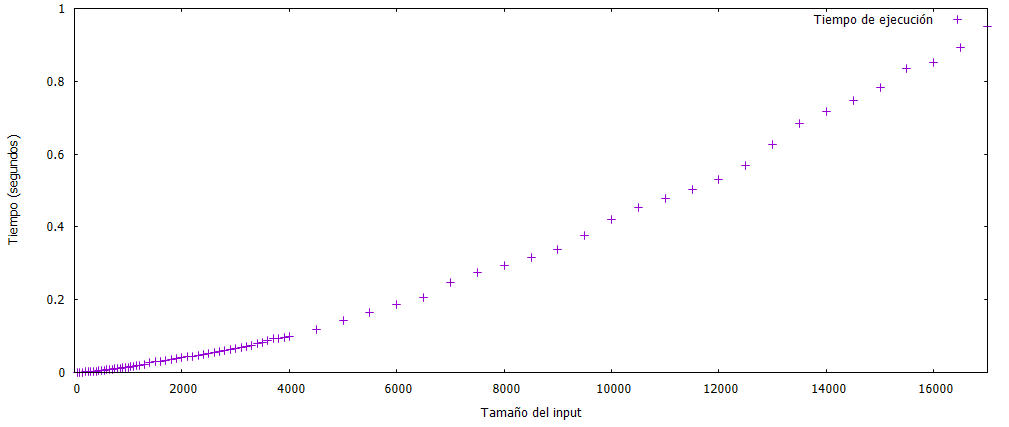
\includegraphics[width=1\textwidth]
   	 	{Imagenes/medianaTiempos.png}
		\caption{Tiempos variando el tama\~no del input}
	\end{figure}
\end{document}